\id{IRSTI 61.01.11}{}
\vspace{1em}
\begin{articleheader}
\sectionwithauthors{L. Tolymbekova, A. Kolpek, E. Kopishev, A. Tursynova, G. Seitenova}{ANALYSIS OF METHODS TO IMPROVE THE STRENGTH AND HEAT RESISTANCE OF COMPOSITE MATERIALS}

{\bfseries
\textsuperscript{1}L. Tolymbekova\alink{https://orcid.org/0000-0002-3785-7943},
\textsuperscript{2}A. Kolpek\alink{https://orcid.org/0000-0003-2809-4574},
\textsuperscript{3}E. Kopishev\alink{https://orcid.org/0000-0002-7209-2341},
\textsuperscript{4}A. Tursynova\alink{https://orcid.org/0000-0001-8957-039X}\textsuperscript{\envelope },
\textsuperscript{5}G. Seitenova\alink{https://orcid.org/0000-0001-6202-395}\textsuperscript{\envelope }
}
\end{articleheader}

\begin{affiliation}
L.N. Gumilev Eurasian National University, Astana, Kazakhstan

\raggedright \textsuperscript{\envelope }Corresponding author: tursynova\_ak@enu.kz, seitenova\_gzh@enu.kz
\end{affiliation}

Modern composites occupy an important place in the production of
high-strength materials due to their lightness, strength, heat
resistance, ability to retain their performance properties and the
possibility of modification for certain tasks. The article presents
modern methods of improving mechanical properties and heat resistance of
metal and polypropylene-based composites, their key characteristics, as
well as modern processing technologies and innovative combinations with
other materials. Particular attention is paid to the prospects for the
development of composites with high temperature resistance through the
introduction of reinforcing refractory particles, the use of carbon
fibers and nanotubes, phosphorus-containing flame retardants, lignin,
elastomers, thermoplastics, which opens up new opportunities for their
exploitation.

Modification of polypropylene using various fillers, such as polyamides,
chalk fillers, and carbon \\nanoparticles, significantly improves its
performance characteristics, including strength, thermal stability, and
electrical conductivity. This opens up new horizons for the use of
polypropylene composites in \\conditions of high loads and high
temperatures, which is important for the sustainable development of the
electronics industry and other high-tech areas.

Metal and polypropylene-based composites have the potential for
application in high temperatures and aggressive environments due to the
possibility of modifying their structure and composition. The methods
and technologies presented in the article allow expanding their
functional capabilities, including integration with innovative
components.

{\bfseries Keywords:} composite materials, heat resistance, polypropylene,
nanocomposites, carbon nanotubes, fibers, thermoplastic elastomers,
adhesion.

\begin{articleheader}
{\bfseries АНАЛИЗ МЕТОДОВ ПОВЫШЕНИЯ ПРОЧНОСТИ И ТЕРМОСТОЙКОСТИ
КОМПОЗИЦИОННЫХ МАТЕРИАЛОВ}

{\bfseries
\textsuperscript{1}Л. Толымбекова,
\textsuperscript{2}А. Колпек,
\textsuperscript{3}Е. Копишев,
\textsuperscript{4}А. Турсынова\textsuperscript{\envelope },
\textsuperscript{5}Г. Сейтенова\textsuperscript{\envelope }
}
\end{articleheader}

\begin{affiliation}
Евразийский национальный университет им. Л. Н. Гумилева, Астана, Казахстан,

e-mail: tursynova\_ak@enu.kz, \href{mailto:seitenova\_gzh@enu.kz}{\nolinkurl{seitenova\_gzh@enu.kz}}
\end{affiliation}

Современные композиты занимают важное место в производстве высокопрочных
материалов благодаря их легкости, прочности, термостойкости, способности
сохранять свои эксплуатационные свойства и возможности модификации под
определенные задачи. В статье представлены современные методы улучшения
механических свойств и термостойкости композитов на основе металла и
полипропилена, их ключевые характеристики, а также современные
технологии обработки и инновационные сочетания с другими материалами.
Особое внимание уделяется перспективам разработки композитов с высокой
термостойкостью за счет введения армирующих тугоплавких частиц,
использования углеродных волокон и нанотрубок, фосфорсодержащих
антипиренов, лигнина, эластомеров, термопластов, что открывает новые
возможности для их эксплуатации.

Модификация полипропилена с использованием различных наполнителей,
таких как полиамиды, меловые наполнители и углеродные наночастицы,
значительно улучшает его эксплуатационные характеристики, включая
прочность, термостойкость и электропроводность. Это открывает новые
горизонты для использования полипропиленовых композитов в условиях
высоких нагрузок и температур, что важно для устойчивого развития
электронной промышленности и других высокотехнологичных областей.

Композиты на основе металлов и полипропилена имеют потенциал для
применения в условиях высоких температур и агрессивных сред благодаря
возможности модификации их структуры и состава. Представленные в статье
методы и технологии позволяют расширить их функциональные возможности, в
том числе за счет интеграции с инновационными компонентами.

{\bfseries Ключевые слова:} композиционные материалы, термостойкость,
полипропилен, нанокомпозиты, углеродные нанотрубки, волокна,
термопластичные эластомеры, адгезия.

\begin{articleheader}
{\bfseries КОМПОЗИЦИЯЛЫҚ МАТЕРИАЛДАРДЫҢ БЕРІКТІГІ МЕН ЫСТЫҚҚА ТӨЗІМДІЛІГІН АРТТЫРУ ӘДІСТЕРІН ТАЛДАУ}

{\bfseries
\textsuperscript{1}Л. Толымбекова,
\textsuperscript{2}А. Көлпек,
\textsuperscript{3}Е. Копишев,
\textsuperscript{4}А. Турсынова\textsuperscript{\envelope },
\textsuperscript{5}Г. Сейтенова\textsuperscript{\envelope }
}
\end{articleheader}

\begin{affiliation}
Л.Н. Гумилев атындағы Еуразия ұлттық университеті, Астана, Қазақстан,

e-mail: tursynova\_ak@enu.kz, seitenova\_gzh@enu.kz
\end{affiliation}

Заманауи композиттер жоғары беріктігі бар материалдарды өндіруде маңызды
орын алады, олардың жеңілдігі, беріктігі, ыстыққа төзімділігі, пайдалану
қасиеттерін сақтау қабілеті және белгілі бір міндеттерге өзгерту
мүмкіндігі. Мақалада металл және полипропилен негізіндегі Композиттердің
механикалық қасиеттері мен ыстыққа төзімділігін жақсартудың заманауи
әдістері, олардың негізгі сипаттамалары, сондай-ақ заманауи өңдеу
технологиялары және басқа материалдармен инновациялық комбинациялар
ұсынылған. Арматуралық отқа төзімді бөлшектерді енгізу, көміртекті
талшықтар мен нанотүтіктерді, құрамында фосфор бар отқа төзімді заттар,
лигнин, эластомерлер, термопластиктерді қолдану арқылы жоғары
температураға төзімді композиттерді әзірлеу перспективаларына ерекше
назар аударылады, бұл оларды пайдаланудың жаңа мүмкіндіктерін ашады.

Полипропиленді полиамидтер, бор толтырғыштары және көміртекті
нанобөлшектер сияқты әртүрлі толтырғыштарды қолдану арқылы өзгерту оның
беріктігін, термиялық тұрақтылығын және электр өткізгіштігін қоса
алғанда, оның өнімділігін айтарлықтай жақсартады. Бұл электронды
өнеркәсіптің және басқа да жоғары технологиялық салалардың тұрақты дамуы
үшін маңызды болып табылатын жоғары жүктемелер мен жоғары температура
жағдайында полипропилен композиттерін қолданудың жаңа көкжиектерін
ашады.

Металдар мен полипропилен негізіндегі Композиттердің құрылымы мен
құрамын өзгерту мүмкіндігіне байланысты жоғары температура мен
агрессивті ортада қолдану мүмкіндігі бар. Мақалада ұсынылған әдістер мен
технологиялар олардың функционалдығын, соның ішінде инновациялық
компоненттермен интеграциялау арқылы кеңейтуге мүмкіндік береді.

{\bfseries Түйін сөздер:} композициялық материалдар, ыстыққа төзімділік,
полипропилен, нанокомпозиттер, көміртекті нанотүтікшелер, талшықтар,
термопластикалық эластомерлер, адгезия.

\begin{multicols}{2}
{\bfseries Introduction.} Modern industry is placing increasingly stringent
demands on materials, especially in areas such as automotive, aerospace
and construction. Traditional materials such as pure metal, plastic or
carbon often cannot meet the requirements for a combination of
lightness, strength and resistance to extreme temperatures. Composite
materials bring out the best properties of different components with
unique characteristics. Improving the mechanical properties and thermal
resistance of composites such as polypropylene, metal and carbon fiber
composites is an important factor in expanding their application and
performance.

Composites are materials made up of two or more components depending on
the natural conditions to achieve a unique advantage. The most widely
used types of composites include polymer, metal and carbon composites.
However, their performance properties are often limited by fragility,
insufficient heat resistance, or poor adhesion between phases {[}1-2{]}.

The main components of composites include matrix (base), responsible for
bonding and dependence, and reinforcing material (filler), increasing
strength and mechanical performance. At the present stage of industrial
development, composites are widely used in a wide variety of fields such
as construction, metallurgy, transportation, medicine, electronics, etc.
{[}3-6{]} The list of main types of composites is diverse and wide.
These are reinforced polymers, composites for pipelines and fittings,
metal matrix composites (MMC), heat resistant composites, carbon fiber
and glass fiber composites, biocomposites, materials for surgical
instruments, etc. {[}7-10{]}.

Current composites have their own problems and limitations, which
includes insufficient interfacial adhesion, brittleness under impact
loading, limited thermal resistance, difficulty in processing and
disposal, initial cost, lack of liquidity data, difficulty in developing
hybrid materials and lack of uniform standard qualities {[}11-13{]}.

Solving these problems requires a comprehensive solution, including the
development of new technologies, optimizing production processes,
improving environmental friendliness and reducing the cost of materials.

Despite this, composites remain in demand due to their excellent
properties, such as high strength, lightness, corrosion resistance and
the ability to create products with specified performance
characteristics. Constant development of technologies, development of
new types of composites and improvement of methods of their production
allow to regulate the scope of their application, reduce costs and
eliminate possible problems.

{\bfseries Materials and methods.} \emph{Metal-based composites.}
Metal-based composites attract great interest. Their structure, which
combines a metallic matrix with inclusions of non-metallic nature,
allows them to overcome the boundaries of high strength, lightness,
corrosion resistance and other unique properties unattainable for
traditional materials. Such properties make them in demand in various
industries including aerospace, automotive, energy and construction
sectors {[}14-16{]}. The most common matrices are aluminum, magnesium,
titanium, and iron. Reinforcing materials can be ceramic particles,
fibers, carbon nanostructures and oxide compounds.

One of the main advantages of metal composites is the ability to
fine-tune their properties by changing their composition and structure.
This is a way to optimize synthesis processes such as powder metallurgy,
mechanical alloying, reinforcement casting and additive technologies.
For example, the addition of carbon nanotubes to an aluminum matrix can
increase the density of a strong material without significantly
increasing its mass {[}17-19{]}.

Special attention is paid to the study of mechanical, thermal and
electrical properties of metal composites, as well as their behavior
under extreme operating conditions. Studies of thermal resistance and
durability open new horizons for the application of materials in
aggressive environments or at high temperatures {[}20-21{]}.

One of the promising structural materials with improved characteristics
are materials obtained by means of various types of reinforcement, such
as metal matrix CMs (composite materials) consisting of a metal or alloy
as a continuous matrix and a reinforcing component in the form of
particles, as well as short or continuous fibers {[}22-26{]}. In metal
matrix CM, the main metal matrices are aluminum, titanium, copper, and
magnesium alloys. According to literature data, in CMs with aluminum
matrix reinforced with carbon fiber, wetting of fibers is carried out to
a sufficient extent, which can improve mechanical properties
{[}27-30{]}.

Metal composites based on titanium matrix have high specific strength
and elastic modulus, high temperature resistance and low density, which
makes them attractive for aerospace, automotive and military
applications, but the use of titanium alloys as structural materials
under conditions of high friction and wear is limited due to their low
tribological properties {[}31-32{]}. Nevertheless, the addition of
refractory particles to titanium and its alloys is an effective way to
improve mechanical and wear properties.

The paper {[}33{]} presents studies on fabrication and evaluation of the
effect of the content of various reinforcing elements on the properties
of metal composite materials (MCMs) based on titanium alloys.
Introduction of refractory particles TiB\textsubscript{2},
B\textsubscript{4}C, SiC and TiC into titanium and its alloys is an
effective way to increase mechanical, wear-resistant and
corrosion-resistant properties with simultaneous reduction of material
density, and also contributes to the expansion of the area of
application of MCMs. The size and distribution of reinforcing particles
in the matrix and their chemical activity have a great influence on the
microstructure and mechanical properties. Carrying out heat treatment
process helps to increase the mechanical properties. Metal composites
reinforced with solid particles have an advantage (compared to MCMs
reinforced with continuous fibers) in the form of isotropic properties,
are cheaper to produce and can be further processed.

In {[}34{]}, the compound B\textsubscript{4}C was used as a reinforcing
element to improve the mechanical, corrosion, and tribological
properties of the titanium alloy of the composition Ti-6Al-4V
(hereinafter referred to as the alloy composition in \% (by mass)),
noting its thermodynamic stability and high mechanical properties. The
alloy of composition Ti- 6Al-4V and ceramic powder B\textsubscript{4}C
with an average particle size of 30 microns were used for the production
of MCM samples by powder metallurgy. MCM samples were made with the
content of 5 and 10 \% (by mass) of B\textsubscript{4}C. As a result of
the study of physical and mechanical properties of the samples, it was
found that the density of MCM decreases with increasing content of
reinforcing particles, but the difference between theoretical and
experimental density increases with increasing B\textsubscript{4}C
content, which is explained by the increase in porosity with increasing
content of B\textsubscript{4}C particles (Fig.1, a). The hardness and
corrosion resistance increase with increasing amount of reinforcing B4C
particles (Fig.1, b).
\end{multicols}

\begin{figure}[H]
	\centering
	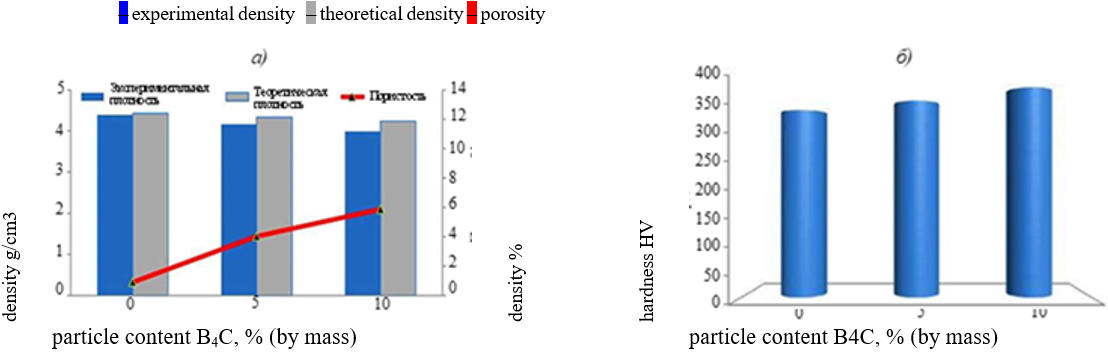
\includegraphics[width=0.8\textwidth]{media/chem4/image11}
	\caption*{Fig.1 - Effect of the content of ceramic B\textsubscript{4}C particles on the properties of MCM composition (Ti-6Al-4V) + B\textsubscript{4}C on density (a) and hardness (b) {[}34{]}}
\end{figure}

\begin{multicols}{2}
Similar studies {[}35-37{]} confirmed that the wear rate of the
composite material decreases with increasing in situ formed TiB and TiC
particles, and concluded that TiB and TiC particles improve the wear
properties of the composite material.

The influence of sintering temperature and the content of
B\textsubscript{4}C particles on the properties of composite material
obtained by powder metallurgy was investigated in {[}38{]}. The increase
in hardness and compressive strength of the composite material increases
with increasing sintering temperature and increasing the content of
reinforcing component.

In {[}39{]} the influence of B\textsubscript{4}C particles and laser
energy density on microhardness of composite material of Ti-6Al-4V
composition obtained by selective laser sintering was investigated. When
obtaining the composite material, B\textsubscript{4}C particles react
with titanium and in the in situ process TiC and TiB particles are
formed in different proportions, the microhardness increases by 30-80 \%
depending on the laser energy density.

Currently, high-modulus carbon fibers are the most suitable material for
creating composites with titanium matrix. Selective reinforcement of
titanium plates of small thickness allows to provide control of high
reactivity of "titanium/carbon" compound and to create suitable
processing methods {[}40-42{]}.

Laminated structures consisting of alternating layers of metal sheets
and fiber-reinforced polymer-matrix composites are also used in aircraft
parts structures. Compared to conventional monolithic metals, they have
high specific strength and stiffness, excellent fatigue resistance
characteristics, and increased fire resistance {[}43{]}.

To improve the mechanical properties of CMs with layered structure,
including metal plastic layer and intermetallic layer (Ti-Al3Ti),
various continuous fibers - carbon (C), silicon carbide (SiC) and
aluminum oxide (Al\textsubscript{2}O\textsubscript{3}) - are introduced.
Using various processing techniques, a number of intermetallic metallic
layered CMs of systems such as Ti-Al, Ni-Al, Nb-Al and Ti-Cu are
obtained. It is believed that the application of such titanium-aluminum
layered CMs with high physical and mechanical properties is potentially
possible in aerospace and armor protection applications. Using a novel
rapid prototyping technique, ultrasonic consolidation was applied to
fabricate three-dimensional structures via additive manufacturing from
metal foil. During the ultrasonic consolidation process, ultrasonic
frequency vibration combined with nominal force was used to generate
static and oscillating shear forces between the metal foil layers that
formed a solid-state bond. Moreover, ultrasonic consolidation was used
to join dissimilar materials such as Ti-Al, Cu-Al, and Fe-Al at low
temperatures (\textasciitilde480 °C). Thus, ultrasonic consolidation can
be used as an auxiliary method to disperse fiber bundles into individual
fibers in the alloy matrix prior to CM formation {[}44-46{]}.

In {[}47{]}, studies were conducted to determine the mechanical
characteristics of CM produced by die casting method using AA6061 matrix
aluminum alloy, which is reinforced with carbon fiber. The studies
showed that increasing the content of reinforcing component from 0 to
10\% (vol.) allows increasing the torque from 24.5 to 52 N-m, tensile
strength from 283 to 315.5 MPa, as well as increasing the impact
strength at 10\% (vol.) of carbon fiber up to 12.2 J {[}47{]}.

The microstructure of the CM of AA6061 grade aluminum alloy and carbon
fiber shows that the carbon fibers are evenly distributed in the matrix,
and interfacial adhesion is present (Figure 2).

\begin{figure}[H]
	\centering
	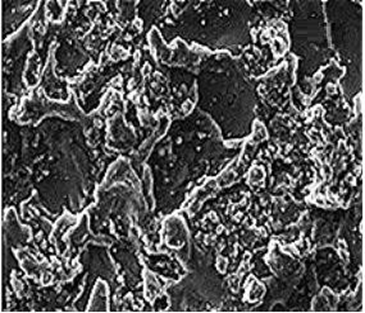
\includegraphics[width=0.8\columnwidth]{media/chem/image8}
	\caption*{Fig.2 - Microstructure of composite material made of aluminum alloy AA6061 and carbon fiber {[}47{]}}
\end{figure}

In similar works {[}48-50{]} the authors describe in detail the physical
and mechanical characteristics of materials with different matrix alloys
(content of reinforcing carbon fibers - from 5 to 50 \% (vol.)) and the
mechanisms of failure of composites after the tests. In {[}48-49{]},
studies of thermophysical and mechanical properties of CMs obtained by
powder metallurgy on the basis of aluminum matrix reinforced with carbon
fibers were carried out. It was found that when the volume content of
carbon fiber increases, hardness, electrical conductivity and strength
decrease: from 71 to 56 HB, from 30.9 to 14.5 cm and from 529 to 214
MPa, respectively, thermal conductivity increases to 155 W/(m-K), and
the temperature coefficient of linear expansion (TCLE) decreases - from
36-10-6 to 8-10-6 K-1 {[}48{]}.

Among the basic properties of composite materials, heat resistance and
heat resistance, the ability of a material to retain its original
strength at high temperature, are of particular importance for the most
common structures {[}51-53{]}. For other types of heat-resistant
materials, such as those based on minerals (ceramics, refractories with
various mineral fillers and binders), the concept of refractoriness is
applicable, i.e. the ability of the material to resist destruction
without deforming during operation at temperatures not lower than 1580
°C {[}54{]}. Composite materials with ceramic matrix have high heat
resistance, relatively high compressive strength, but tensile strength
and impact strength have low values. The scientific direction of solving
the problem of increasing the strength of composite material is the
necessity of transferring a significant part of the load to reinforcing
elements {[}55-57{]}.

It is of scientific and practical interest to solve the problem of
increasing the strength and heat resistance of composite material of the
metal-ceramic system by changing the macrostructure of the introduced
reinforcing material and matrix composition.

The most common methods of molding composite materials are pressing and
sintering, which in some cases is not economical, for example, molds are
difficult to manufacture, this disadvantage significantly increases the
cost of products. The use of slurry with hydrophilic tooling to remove
moisture and give primary technological strength to the composite
material, provides cost reduction and increased cost-effectiveness
{[}58-60{]}.

In work {[}61{]}, the analysis of properties of composite materials is
given, increase of heat resistance and heat resistance of composite
material on the basis of stabilized silica, wastes of metallurgical and
glass industries, was achieved by improving the structure of composite
material, introduction of reinforcing elements. For the production of
composite material was used an economical method of molding into
hydrophilic tooling.

Slip is a suspension in the form of liquid dispersion medium and solid
fine-dispersed phase, for example, in the form of SiO2 and Fe, crushed
to the size of 0.5...10 microns, as well as additives: stabilizing
volumetric transformations of SiO2 during heating or cooling (Na2O);
increasing sedimentation stability of slip (refractory clay). This
material is fluid in the stage of preparation and pouring, plasticity
while in the mold and strength after partial dehydration of the slip,
for example, in a gypsum mold. The combination of stabilized
silica-based slurry, reinforcing components, glass production waste and
hydrophilic tooling reduces energy consumption by 18\% and increases the
cost-effectiveness of manufacturing products of the metal-ceramic system
in comparison with traditional methods of composite materials forming
{[}61{]}.

Despite the obvious advantages, the development of metal-based
composites involves obtaining a criterion for uniform distribution of
reinforcing particles and the need to accurately determine the
interactions between components. However, modern advances in computer
modeling, nanotechnology, and experimental techniques offer new
opportunities to overcome these difficulties. Thus metal-based
composites continue to be the basis of research that will shape the
development of high-tech materials in the future. Their unique
properties and potential applications in a wide range of regions make
them the object of close attention of the scientific community and
industry.

\emph{Polypropylene-based composites.} Today, polymer composites are of
particular interest and are being actively introduced into various
fields due to their unique properties, including high elasticity,
strength, stiffness and high specific strength.

Polypropylene is one of the most widely used polymers in the world.
Since its commercial introduction in the 1950s, polypropylene has
established a reputation for its unique properties and versatility in
application {[}62{]}.

Polypropylene can be easily molded and extruded to produce complex
shapes. It is able to retain its size and shape when exposed to high
temperatures and loads. It combines low density and high strength,
making it ideal for use in the manufacture of lightweight but strong
products {[}63{]}.

Modern technologies make it possible to combine polypropylene with
natural and synthetic fibers. This opens up new possibilities for
creating materials with improved thermal and mechanical properties. The
addition of synthetic fibers and fillers (such as carbon or glass
fibers) can improve the strength and stiffness of polypropylene
products, which expands their application {[}64{]}.

The improvement of these materials through the addition of carbon
nanotubes (CNTs) and fibers is an active area of research aimed at
improving their performance {[}65{]}.

Modification of polypropylene with carbon nanotubes and fibers allows to
significantly improve the mechanical properties of composites, in
particular, their impact resistance and stiffness. It was found that the
addition of carbon nanotubes can increase the impact resistance of the
composite up to seven times, which makes such materials competitive with
more expensive analogs. Mechanical stiffness and resistance to
deformation under load are also significantly increased by the inclusion
of continuous carbon fibers, which expands their application areas,
including high and low temperature conditions {[}66{]}.

The need to use carbon nanotubes arises due to their unique properties,
including high thermal conductivity, strength and the ability to form
conductive networks within the polypropylene structure. Studies show
that the introduction of CNTs into PP composites leads to a significant
improvement in mechanical properties due to a more homogeneous
distribution of reinforcing additives and their strong interaction with
the polymer matrix {[}67{]}.

Many CNT modification techniques, including covalent and non-covalent
modification, are used to achieve the best results in the creation of
composites. These methods help to improve the dispersion of fillers in
the polymer matrix, allowing for more robust interfacial interactions.
CNT modification allows the attachment of functional groups such as
epoxy, hydroxyl and carboxyl groups, which also helps to improve the
bond strength between the matrix and filler {[}68{]}.

In addition, oxidation of carbon nanotubes carried out using various
oxidizing agents such as H₂SO₄, KMnO₄, H₂O₂ and HNO₃ allows the
introduction of functional groups on their surface. This leads to the
formation of defective sites, which can adversely affect the engineering
properties, but this approach significantly improves the adhesion of
CNTs in the polymer matrix, which is the cornerstone of an efficient
composite structure {[}69{]}.

The introduction of nanotubes into the structure of polypropylene
composites provides improvements in properties such as strength, heat
resistance and mechanical stiffness, making them competitive with more
expensive materials {[}70{]}.

Studies show that PP and nanotube-based composites exhibit significant
improvements in mechanical properties such as impact resistance and
stiffness. Carbon nanotubes contribute to increased strength and
resistance to deformation under loading due to their high strength and
ability to form conductive networks within the polymer matrix. In
particular, the use of metallocene polypropylene in combination with
carbon fillers improves the strength and ductility of composites
{[}71{]}.

Melt extrusion is the preferred method of producing PP-CNT composites
because of its ability to create homogeneous materials through mixing of
components at high temperatures. However, lack of control during the
extrusion process can lead to thermal fracture and residual stresses
that negatively affect the properties of the composites. To increase the
dispersion of CNTs in the polymer matrix, various modifications and
blending methods are actively investigated, indicating the importance of
controlling the extrusion process to achieve optimal performance
{[}72{]}.

Modifications of carbon nanotubes are necessary to ensure high-quality
interfacial adhesion between PP and CNTs. The grafting of maleic
anhydride (MA) onto polymer chains significantly improves the
compatibility of CNTs with the polymer matrix and also helps to reduce
the surface tension. This allows for better dispersion of CNTs and
formation of efficient percolation networks. Studies show that the use
of modified compatibilizers such as styrene-ethylene/butylene-styrene
copolymer leads to a significant improvement in the mechanical and
thermal properties of composites {[}73{]}.

The high flammability of polypropylene limits its use in applications
requiring fire resistance. To solve this problem, active research is
directed to the use of phosphorus-containing flame retardants
(phosphorus fire retardant additives), which show high efficiency in
reducing the flammability of polymeric materials {[}74{]}.

Phosphorus flame retardants have unique properties that provide low
toxicity and the ability to form a protective layer on the surface of
the material when exposed to high temperatures. This protective layer
promotes thermal decomposition of the flame retardant, forming a carbon
residue that serves as a barrier to flame propagation. These mechanisms
of action make it possible to significantly increase the fire resistance
of polypropylene composites {[}75{]}.

Studies conducted by various research groups have confirmed that the
addition of phosphorus flame retardants to PP significantly improves its
mechanical and thermal properties. The addition of phosphorus flame
retardants to PP increases the tensile strength and stiffness of
composites at high temperatures, which improves their performance
without degrading the basic properties {[}76{]}.

Phosphorus-containing flame retardants are a promising alternative to
halogen-containing flame retardants, which were previously widely used
but criticized for their toxicity and negative environmental impact. In
contrast, phosphorus-containing additives help to reduce flammability
while remaining safer for humans and nature {[}77{]}.

The retrofitting of polypropylene with phosphorus-containing flame
retardants opens new horizons for the application of composites in
products that require high fire resistance. For example, the study of
new methods of modifying composites, such as blending with carbon
nanotubes (CNTs), improves thermal stability and mechanical properties
while maintaining environmental safety {[}78{]}.

To achieve higher performance characteristics of polypropylene
composites with phosphorus-containing flame retardants, it is necessary
to continue the optimization of compositions and technologies of their
processing. This includes the study of new polymer modifications and the
use of alternative fillers, which can lead to the creation of stable and
functional materials that meet modern requirements {[}79{]}.

Polypropylene is one of the most popular thermoplastics with good
mechanical and physical properties. However, various modification
methods are being investigated to enhance its functionality and
performance, including the use of biopolymers such as lignin and
chitosan. These additives not only improve the mechanical properties of
composites but also make them more environmentally friendly {[}80{]}.

Modification of polypropylene with chitosan fibers can significantly
improve its strength and impact resistance. Chitosan, being a biopolymer
with good adhesion to the polymer matrix, contributes to the improvement
of tensile and impact performance. Experiments have demonstrated that
composites with modified fibers provide a significant improvement in
mechanical properties compared to unmodified samples {[}81{]}.

The use of esterified lignin as a modifier is important for achieving
high adhesion between composite components. Lignin, being a secondary
natural polymer, shows excellent binding properties, which improves the
structure of the final material. Studies show that the presence of
lignin helps to create strong interfacial interactions between chitosan
and polypropylene, which enhances the strength and durability of the
composite {[}82{]}.

The process of mixing the components at high temperatures, such as
190°C, ensures uniform distribution of fillers in the polypropylene
matrix. Homogeneity of distribution is critical to achieving optimum
strength and strain resistance. Studies in this area show that lack of
homogeneity can lead to poor mechanical performance and reduced material
stability {[}83{]}.

The resulting polypropylene-based composites with modifiers such as
lignin and chitosan have a wide range of potential applications in
industries such as packaging and construction. These fields require
lightweight and strong materials that can withstand mechanical stresses.
The improved performance of modified composites opens up new
opportunities for their use in various sectors including automotive and
consumer products {[}84{]}.

Composites based on thermoplastic elastomers have attracted considerable
attention due to their unique properties that provide high flexibility,
strength and resistance to external influences. Of particular interest
is the combination of styrene thermoplastic elastomers with
polypropylene, which makes them promising for applications in the
construction industry and other areas where high strength and durability
of materials are required {[}85{]}.

Thermoplastics are classes of polymers that combine the properties of
thermoplastics and elastomers. They are recyclable, making them
convenient for manufacturing processes, while providing the elasticity
characteristic of rubber bands. Studies show that blends of styrene
thermoplastic elastomers and polyolefin elastomers can improve the
performance of materials, which has initiated a number of scientific
studies in this area {[}86{]}.

One of the key tasks in improving composites based on thermoplastic
elastomers is to increase their resistance to thermal oxidative
degradation. Studies show that the introduction of antioxidants,
heat-resistant fillers and modifiers can significantly improve the
performance characteristics of materials and their durability {[}87{]}.

Improving the fire resistance of thermoplastic elastomers is also an
important aspect for their use in building structures. The use of
minerals such as aluminum hydroxide and other flame-retardant additives
shows promising results in improving the fire-retardant properties of
composites, making them safer for use in high temperature environments
{[}88{]}.

The problem of rubber waste utilization remains relevant, and the use of
crumb rubber as a filler for thermoplastics provides an opportunity not
only to solve environmental problems, but also to expand the application
area of such composites. Studies have proven that the addition of crumb
rubber to polyethylene and polypropylene can improve certain mechanical
characteristics such as impact strength and flexibility {[}89{]}.

The key factors affecting the mechanical properties of composites are
matrix characteristics, filler particle size and the level of adhesion
between components. Optimization of these properties can be achieved by
various methods such as changing the mixing technology, using modifiers
and adhesion promoters {[}90{]}.

The study of composites based on thermoplastic elastomers, particularly
their blends with polypropylene and styrene thermoplastic elastomers,
has become an important aspect because of the increasing demands for
durability and safety of building materials {[}91{]}.

Thermoplastic elastomers, including blends with polyolefin elastomers,
have flexible, strong and resistant properties. This allows them to find
applications in the construction, medical and automotive industries,
where high strength and durability of materials are required {[}92{]}.

Also the practical significance of the research lies in the development
of new formulations of composites based on thermoplastic elastomers,
which allows to create materials with improved performance
characteristics. The created composites are characterized by high
resistance to thermo-oxidative degradation and reduced flammability,
which makes them suitable for the production of window seals, cable
products, roofing membranes and other construction products {[}93{]}.

The introduction of crumb rubber into the composition of thermoplastics
solves the problems of utilization of waste rubber products and expands
the practical applications of plastics. The resulting rubber plastics
are used in waterproofing, production of roofing materials and rubber
tiles, while optimizing their mechanical properties {[}94{]}.

Studies show that different temperatures and rubber filler content
significantly affect the deformation and strength of composites. In
particular, certain concentrations of crumb rubber contribute to the
transition of the material from brittle fracture to macrouniform plastic
deformation, which opens up opportunities for targeted modification of
the properties of rubber plastics {[}95-96{]}.

Incorporation of waste-derived graphene into polymer composites can
increase their mechanical and thermal performance while improving
flexural and tensile strength. This supports the trend towards lighter
and greener materials, which helps to reduce the carbon footprint in the
automotive and other industries {[}97{]}.

{\bfseries Results and Discussion.} Research into polymers with improved
conductive properties opens new horizons for flexible electronics. The
development of conductive polymer nanocomposites can contribute to the
creation of more reliable and durable flexible electronic devices, which
will be a significant step forward in technology development {[}98{]}.

Modification of polypropylene using various fillers such as polyamides,
chalk fillers and carbon nanoparticles significantly improves its
performance characteristics including strength, thermal stability and
electrical conductivity. This opens new horizons for the application of
polypropylene composites in high stress and high temperature
environments, which is important for the sustainable development of the
electronics industry and other high-tech fields {[}99{]}.

Research and development of polypropylene-based nanocomposites using
various fillers open new horizons in the construction industry,
improving the mechanical characteristics and thermal stability of
materials. Special fillers help to accelerate crystallization processes
and increase resistance to environmental influences, which makes such
composites competitive for use not only in construction, but also in the
packaging and automotive industries {[}100{]}.

Thus, polypropylene composites are a promising area in materials
production due to their versatility, availability and modification
possibilities, such as carbon nanotubes, phosphorus-containing flame
retardants, lignin, elastomers, thermoplastics and others. These
modifications allow to significantly improve mechanical properties, heat
resistance, flame retardancy and expand their application in high-tech
and industrially important areas.

{\bfseries Conclusions.} Research in the field of increasing the strength
and heat resistance of composite materials is one of the promising areas
in the field of chemical technologies and materials science, opening up
wide opportunities for the development of innovative solutions.

Metal and polypropylene-based composites have the potential for
application in high temperatures and aggressive environments due to the
possibility of modifying their structure and composition. The methods
and technologies presented in the article allow expanding their
functional capabilities, including integration with innovative
components.

The review shows that the use of modern modification methods, such as
the introduction of reinforcing refractory particles, improvement of
interfacial interaction, the use of carbon fibers and nanotubes,
phosphorus-containing flame retardants, lignin, elastomers,
thermoplastics allows to significantly increase the strength
characteristics and heat resistance of composites.

The prospectivity of developments in this direction is due to the
growing requirements for materials used in the metallurgical industry,
construction, transportation, energy. Special attention should be paid
to the development of hybrid materials that combine the advantages of
polymers, metals and carbon fibers. Future research should be aimed at
optimizing upgrading technologies and studying their performance
characteristics of composites.

\emph{{\bfseries Funding:} BR24992883 Establishment of a science and
technology park for petrochemicals and polymer materials to provide
services and implementation of applied Research Work results in priority
sectors of the country' s economy (2024-2026).}
\end{multicols}

\begin{center}
{\bfseries References}
\end{center}

\begin{references}
1.  Kolosova A.S., Sokolskaya M.K., Vitkalova I.A. Sovremennye
polimernye kompozicionnye materialy i ih primenenie // Mezhdunarodnyj
zhurnal prikladnyh i fundamental'nyh issledovanij. - 2018. - No. 5. -
S. 245–256. URL: \href{https://applied-research.ru/ru/article/view?id=12252&ysclid=m7kors1qru673331574}{https://applied-research.ru}.

2. Sokolskaya M.K., Kolosova I.A., Vitkalova A.S. Svjazujushhie dlja
poluchenija sovremennyh polimer\-nyh kompozicionnyh materialov //
Fundamental'nye issledovanija – 2017. – № 10-2. – S. 290 –
295. URL: \href{https://fundamental-research.ru/ru/article/view?id=41827&ysclid=m7kowxw7wd681574555}{https://fundamental-research.ru}.

3. Gurbanov N.A., Sidorov D.B., Ismailova K.H. Composite materials,
general properties and usage areas // Sciences of Europe. – 2021. – №
78. – . 25-27. DOI 10.24412/3162-2364-2021-78-1-25-27.

4. Hull D., Clyne T.W. An Introduction to Composite Materials. –
Cambridge: Cambridge University Press, 1996. – 326 p. ISBN
978-0521388559. \href{https://doi.org/10.1017/CBO9781139170130}{https://doi.org}.

5. Schwartz M.M. Composite Materials: Properties, Non-Destructive
Testing and Repair, Polymer, Cera\-mic, Metal Matrices. – USA: Prentice
Hall Inc., 1997. – 423
p. URL: \href{https://openlibrary.org/books/OL990224M/Composite_materials}{https://openlibrary.org}.

6. Chernyshov E.A., Romanov A.D. Sovremennye tehnologii izgotovlenija
izdelij iz kompozicionnyh materialov // Sovremennye naukoemkie
tehnologii. – 2014. – No. 2. –
S. 45–51. URL: \\\href{https://s.top-technologies.ru/pdf/2014/2/33649.pdf}{https://s.top-technologies.ru}.

7. Rogov V.A., Shkarupa M.I., Velis A.K. Klassifikacija kompozicionnyh
materialov i ih rol' v sovremen\-nom mashinostroenii // Vestnik
RUDN. Serija Inzhenernye issledovanija – 2012. – No. 2. –
P. 41–49. URL: \href{https://journals.rudn.ru/engineering-researches/article/view/4839?ysclid=m6j2ggf0is563072114}{https://journals.rudn.ru}.

8. Karabasov Y.S. Novye materialy. – Moskva: Izdatel'stvo
MISIS. 2002. – 738 s. ISBN
5-87623-114-2. \href{https://search.rsl.ru/ru/record/01001838887?ysclid=m87kojnf2s394686147}{https://search.rsl.ru}.

9. Popov A. Ju., Gosija K. K., Petrov I. V. Klassifikacija, sostav,
preimushhestva i nedostatki mnogokomp\-onentnyh kompozicionnyh
materialov // Omskij nauchnyj vestnik. – 2015. – № 3 (143). –
S. 42-45. \href{https://elibrary.ru/vcntut?ysclid=m6j2mhco63336644284}{https://elibrary.ru}.

10. Wanberg J. Composite Materials: Fabrication Handbook \#2. – USA:
Wolfgang Publications, Inc., 2010. – 144 p. ISBN
1929133936. \href{https://www.librarything.com/work/9709968}{https://www.librarything.com}.

11. Jah'jaeva H.Sh ., Zajkov G.E., Deberdeev T.R., Ulitin
N.V. Strukturnye osnovy mezhfaznoj adgezii v polimernyh kompozitah //
Vestnik Kazanskogo tehnologicheskogo universiteta. – 2012. – Tom 15, №
5. – S. 68-70.
\href{https://cyberleninka.ru/article/n/strukturnye-osnovy-mezhfaznoy-adgezii-nanoadgezii-v-polimernyh-kompozitah?ysclid=m6j2st57s6418214983}{https://cyberleninka.ru}. 

12. Smirnova O.E., Pichugin A.P., Hritankov V.F. Adgezionnaja
prochnost' v strukture kompozicionnyh materialov na osnove
organicheskogo syr'ja. Stroitel'nye materialy. 2024. №
5. S. 17-21. \href{https://doi.org/10.31659/0585-430X-2024-824-5-17-21}{https://doi.org}.

13. Mel'nichenko M. A., Ershova O. V., Chuprova L. V. Vlijanie sostava
napolnitelja na svojstva polimer\-nyh kompozicionnyh materialov. Molodoj
uchenyj. № 16 (96),
2015. S. 199-202. \href{https://moluch.ru/archive/96/21554/}{https://moluch.ru}.

14. Milejko S.T. Novye kompozity s metallicheskoj
matricej. Mezhotraslevoj seminar pamjati prof. T.D. Karimbaeva
"Primenenie kompozicionnyh materialov v dvigatelestroenii", Moskva,
Rossija, 2023/
S. 7-10. \href{https://ciam.ru/composites_theses/mileiko.pdf}{https://ciam.ru}.

15. Ivanov V.A. Metody vosstanovlenija tehnologicheskogo i
vspomogatel'nogo oborudovanija iznoso\-stojkimi kompozicionnymi
materialami. Dissertacija na soiskanie uchenoj stepeni kandidata
tehnicheskih nauk. Moskva - 2014. 166
s. \href{https://new-disser.ru/_avtoreferats/01007923651.pdf?ysclid=m6j2zfwyqg324913287}{https://new-disser.ru}.

16. Milejko S.T. Jentoni Kelli i kompozitnye materialy
segodnja. Chast' 2: Kompozity s metallicheskoj matricej // Kompozity i
nanostruktury. 2021. Tom 13, № 3-4
(51-52). S. 59-107. DOI:10.36236/1999-7590-2021-13-3-4-59-107. \href{https://www.elibrary.ru/item.asp?id=48118660&ysclid=m87loyv5gc289218394}{https://www.elibrary.ru}.

17. Senjushkin N.S., Jamaliev R.R., Jalchibaeva L.R. Primenenie
kompozicionnyh materialov v konstrukcii bespilotnyh letatel'nyh
apparatov // Molodoj uchenyj. 2011. № 4 (27). Tom
1. S. 59-61. \href{https://moluch.ru/archive/27/2963/?ysclid=m6j31n5ru1840809790}{https://moluch.ru}.

18. Even C., Arvieu C., Quenisset J.M. Powder route processing of
carbon fibers reinforced titanium matrix composites // Composites
Science and Technology. 2008. Vol. 68,
Iss. 6. P. 1273-1281. 1273-1281. DOI:10.1016/j.compscitech.2007.12.014. \href{https://hal.science/hal-00550280/document}{https://hal.science}.

19. Saldias C., Bonardd S., Quezada C., Radic D., Leiva A. The role of
polymers in the synthesis of noble metal nanoparticles: a review //
Journal of Nanoscience and
Nanotechnology. 2017. Vol. 17. P. 87-114. http://dx.doi.org/10.1166/jnn.2017.13016. \href{https://www.researchgate.net/publication/302927159_The_Role_of_Polymers_in_the_Synthesis_of_Noble_Metal_Nanoparticles_A_Review}{https://www.researchgate.net}.

20. Prokopec A. D., Bazin P.M., Konstantinov A.S., Chizhikov
A.P. Struktura i mehanicheskie harakteris\-tiki sloistogo
kompozicionnogo materiala na osnove magnetronnoj fazy Ti3AlC2,
poluchennogo metodom svobodnogo SVS-szhatija // Neorganicheskie
materialy. 2021. Tom 57, №
9. S. 986-990. \href{https://doi.org/10.31857/S0002337X2109013X}{https://doi.org}.

21. Sabadaha E.N., Prokopchuk N.R., Shutova A.L. Termostabil'nye
kompozicionnye materialy // Trudy BGTU. 2017. Serija 2, №
2. S. 108-115. \href{https://cyberleninka.ru/article/n/termostabilnye-kompozitsionnye-materialy/viewer}{https://cyberleninka.ru}.

22. Grashhenkov D.V. Strategija razvitija nemetallicheskih materialov,
metallicheskih kompozicionnyh materialov i teplozashhity //
Aviacionnye materialy i tehnologii. 2017. № S. S. 264-271. DOI:
10.18577 /2071 -9140 -2017 -0 -S -264
-271. \href{https://cyberleninka.ru/article/n/strategiya-razvitiya-nemetallicheskih-materialov-metallicheskih-kompozitsionnyh-materialov-i-teplozaschity?ysclid=m82pcgt3m5269227216}{https://cyberleninka.ru}.

23. Akmeev A.R., Guljaev I.N., Il'ichev A.V., Ivanov N.V. Issledovanie
mehanicheskih svojstv metallok\-ompozita (Aljuminij-ugleplastik) s
adaptivnoj shemoj armirovanija // Aviacionnye materialy i
tehnologii. 2017. № 3 (48). S. 43-49. DOI: 10.18577 /2071 -9140 -2017
-0 -3 -43
-49. \href{https://www.elibrary.ru/item.asp?id=29728812&ysclid=m87lxlwmk6845840919}{https://www.elibrary.ru}.

24. Jakovlev A.L., Nochovnaja N.A., Putyrskij S.V., Krohin
V.A. Titanopolimernye sloistye materialy // Aviacionnye materialy i
tehnologii. 2016. № S2 (44). S. 56-62. DOI: 10.18577 /2071 -9140 -2016
-0 -S2 -56
-62. \href{https://www.elibrary.ru/item.asp?id=27022904&ysclid=m87m1shkiq269457456}{https://www.elibrary.ru}.

25. Arislanov A.A., Goncharova L.Ju., Nochnaja N.A., Goncharov
V.A. Perspektivy ispol'zovanija titan\-ovyh splavov v sloistyh
kompozicionnyh materialah // Trudy VIAM. 2015. №
10. S. 20-23. \href{https://dx.doi.org/10.18577/2307-6046-2015-0-10-4-4}{https://dx.doi.org}. \href{https://cyberleninka.ru/article/n/perspektivy-ispolzovaniya-titanovyh-splavov-v-sloistyh-kompozitsionnyh-materialah/viewer}{https://cyberleninka.ru}.

26. Valueva M.I., Zelenina I.V., Haskov M.A., Guljaev A.I. Poluchenie
uglerodnogo volokna dlja mezhfaz\-nogo pokrytija kompozicionnyh
materialov s keramicheskoj matricej // Trudy VIAM. 2017. № 10
(58). S. 79-89. \href{https://doi.org/10.18577/2307-6046-2017-0-10-9-9}{https://doi.org}.

27. Mahaviradhan N., Sivaganesan S., Sravya N.P., Parthiban
A. Experimental investigation on mechanical properties of carbon fiber
reinforced aluminum metal matrix composite // Materials Today:
Proceedings. 2021. Vol. 39, Part
1. P. 743-747. \href{http://dx.doi.org/10.1016/j.matpr.2020.09.443}{http://dx.doi.org}.

28. Deshpande M., Gondil R., Rahul S.V.S., et al. Processing and
characterization of carbon fiber reinforced aluminium 7075 //
Materials Today: Proceedings. 2018. Vol. 5
(2). P. 7115-7122. \\\href{http://dx.doi.org/10.1016/j.matpr.2017.11.376}{http://dx.doi.org}. \href{https://www.researchgate.net/publication/312780136_Processing_of_Carbon_fiber_reinforced_Aluminium_7075_metal_matrix_composite}{https://www.researchgate.net}.

29. Deshpande M., Ramesh S.V.S., Gondil R., et al. Studies on 7075
aluminum alloy MMCs with milled carbon fibers as reinforcements //
Transactions of the Indian Institute of Metals. 2018. Vol. 71
(4). P. 993-1002. \href{https://doi.org/10.1007/s12666-017-1233-4}{https://doi.org}.

30. Tamilarasan U., Karunamoorthy L., Palanikumar K. Mechanical
properties evaluation of the carbon fiber reinforced aluminum sandwich
composites // Materials Research. 2015. Vol. 18
(5). P. 1029-1037. http://dx.doi.org/10.1590/1516-1439.017215. \href{https://www.researchgate.net/publication/283618484_Mechanical_Properties_Evaluation_of_the_Carbon_Fibre_Reinforced_Aluminium_Sandwich_Composites}{https://www.researchgate.net}.

31. Tian Y.S., Chen C.Z., Chen L.B., Liu J.H. Wear properties of
alloyed layers produced by laser surface alloying of pure titanium
with B4C and Ti mixed powders // Journal of Materials
Science. 2005. No. 40. P. 4387-4390. \href{https://link.springer.com/article/10.1007/s10853-005-0736-2}{https://link.springer.com}.

32. Fouvry S., Paulin C., Deyber S. Impact of contact size and complex
gross-partial slip conditions on Ti-6Al-4V/Ti-6Al-4V fretting wear //
Tribology International. – 2009. – Vol. 42, Is. 3. – P. 461–474. DOI:
10.1016/j.triboint.2008.08.005. \href{https://www.sci-hub.ru/10.1016/j.triboint.2008.08.005?ysclid=m87mkr00fc385128516}{https://www.sci-hub.ru}.

33. Krasnov E.I., Serpova B.M., Hodykin L.F., Gololobov
A.B. Metallicheskie kompozicionnye materialy na osnove titanovyh
splavov, armirovannyh tugoplavkimi chasticami (Obzor) // Trudy VIAM. –
2021. – № 6 (100). –
S. 36-45. \href{https://dx.doi.org/10.18577/2307-6046-2021-0-6-36-45}{https://dx.doi.org}.

34. Soorya Prakash K., Gopal P.M., Anburose D., Kavimani
V. Mechanical, corrosion and wear character\-istics of powder metallurgy
processed Ti-6Al-4V/B4C metal matrix composites // Ain Shams
Engineering Journal. – 2018. – Vol. 9, Is. 4. –
P. 1489–1496. \href{https://doi.org/10.1016/j.asej.2016.11.003}{https://doi.org}.

35. Qin Y.L., Geng L. Dry sliding wear behavior of titanium matrix
composites hybrid-reinforced by in situ TiB whisker and TiC particle
// Journal of Materials Science. – 2011. – Vol. 46, No. 14. –
P. 4980–4985. DOI:
10.1007/s10853-011-5415-x. \href{https://link.springer.com/article/10.1007/s10853-011-5415-x}{https://link.springer.com}.

36. Balaji V.S., Kumaran S. Dry sliding wear behavior of titanium (TiB
+ TiC) in situ composite developed by spark plasma sintering //
Tribology Transactions. – 2015. – Vol. 58, Is. 4. – P. 698–703. DOI:\\
10.1080/10402004.2014.993780. \href{https://www.researchgate.net/publication/276508350_Dry_Sliding_Wear_Behavior_of_Titanium-TiBTiC_in_situ_Composite_Developed_by_Spark_Plasma_Sintering}{https://www.researchgate.net}.

37. Zheng B., Dong F., Yuan X. et al. Microstructure and tribological
behavior of in situ synthesized (TiB + TiC)/Ti6Al4V (TiB/TiC = 1/1)
composites // Tribology International. 2020. Vol. 145. Reference
106177. DOI:
10.1016/j.triboint.2020.106177. \href{https://www.sci-hub.ru/10.1016/j.triboint.2020.106177?ysclid=m836h762qf658864232}{https://www.sci-hub.ru}.

38. Yoganandam K., Mohanavel V., Vijayakumar M.D.,
V. KannadhasanMechanical properties of titanium matrix composites
fabricated via powder metallurgy method // Materials Today:
Proceedings. 2020. P. 5-10. \href{https://doi.org/10.1016/j.matpr.2020.04.569}{https://doi.org}.

39. Fereiduni, E. Selective laser melting of hybrid ex-situ/in-situ
reinforced titanium matrix composites: Laser/powder interaction,
reinforcement formation mechanism, and non-equilibrium microstructural
evo\-lutions / E. Fereiduni, A. Ghasemi, M. Elbestawi // Materials \&
Design. – 2019. – Vol. 184. –
Ref. 108185. \href{https://doi.org/10.1016/j.matdes.2019.108185}{https://doi.org}.

40. Even, C. Powder route processing of carbon fibers reinforced
titanium matrix composites / C. Even, C. Arvieu, J.M. Quenisset //
Composites Science and Technology. – 2008. – Vol. 68. –
P. 1273–1281. \href{http://dx.doi.org/10.1016/j.compscitech.2007.12.014}{http://dx.doi.org}. \href{https://hal.science/hal-00550280v1}{https://hal.science}.

41. Arvieu, C. Interaction between titanium and carbon at moderate
temperatures [Text] / C. Arvieu, J.P. Manaud, J.M. Quenisset //
Journal of Alloys and Compounds. – 2004. – Vol. 68. –
P. 116–122. \href{http://dx.doi.org/10.1016/j.jallcom.2003.08.051}{http://dx.doi.org}.

42. Sidorov, D.V. Issledovanie mezhfaznogo vzaimodejstvija na granice
razdela v sisteme Ti-C s otechestv\-ennymi titanovymi splavami α+β i
psevdo-α klassov [Tekst] / D.V. Sidorov, V.M. Serpova, A.V. Zavodov,
A.A. Shavnev // Fizika i himija obrabotki materialov. – 2020. – № 5. –
S. 75-81. \href{https://doi.org/10.30791/0015-3214-2020-5-75-81}{https://doi.org}.

43. Jiao, F. Continuous carbon fiber reinforced Ti/Al3Ti
metal-intermetallic laminate (MIL) composites fabricated using
ultrasonic consolidation assisted hot pressing sintering [Text] /
F. Jiao, M. Liu, F. Jiang [et al.] // Materials Science \& Engineering
A. – 2019. – Vol. 765. –
P. 1–21. \href{http://dx.doi.org/10.1016/j.msea.2019.138255}{http://dx.doi.org}. \\\href{https://www.sciencedirect.com/science/article/abs/pii/S092150931931041X?via\%3Dihub}{https://www.sciencedirect.com}.

44. Han, Y. Fabrication, interfacial characterization and mechanical
properties of continuous Al2O3 cera\-mic fiber reinforced Ti/Al3Ti
metal-intermetallic laminated (CCFR-MIL) composite / Y. Han, C. Lin,
X. Han [et al.] // Materials Science \& Engineering A. – 2017. –
Vol. 688. –
P. 338–345. \href{http://dx.doi.org/10.1016/j.msea.2017.02.024}{http://dx.doi.org}. \href{https://www.sciencedirect.com/science/article/abs/pii/S0921509317301818?via\%3Dihub}{https://www.sciencedirect.com}.

45. Ji. C., Wang. B., Hu. J., et al. Effect of different preparation
methods on mechanical behaviors of carbon fiber-reinforced
PEEK-Titanium hybrid laminates // Polymer Testing. – 2020. –
Vol. 85. – P. 1–10. Corresponding
author. \href{https://doi.org/10.1016/j.polymertesting.2020.106462}{https://doi.org}. \href{https://www.sci-hub.ru/10.1016/j.polymertesting.2020.106462?ysclid=m839czkw50582004401}{https://www.sci-hub.ru}.

46. Vecchio, K.S., Jiang, F. Fracture toughness of
Ceramic-Fiber-Reinforced Metallic-Intermetallic-Lami\-nate (CFR-MIL)
composites // Materials Science \& Engineering A. – 2016. –
Vol. 649. –
P. 407–416. \href{https://doi.org/10.1016/j.msea.2015.10.018}{https://doi.org}. \href{https://www.sciencedirect.com/science/article/abs/pii/S0921509315304822?via\%3Dihub}{https://www.sciencedirect.com}.

47. Mahaviradhan, N., Sivaganesan, S., Sravya, N.P., Parthiban,
A. Experimental investigation on mechan\-ical properties of carbon fiber
reinforced aluminum metal matrix composite // Materials Today:
Proceed\-ings. – 2021. – Vol. 39, Part 1. –
P. 743–747. https://doi.org/10.1016/j.matpr.2020.09.443. \href{https://www.sci-hub.ru/10.1016/j.matpr.2020.09.443?ysclid=m839ktt5c4169456263}{https://www.sci-hub.ru}.

48. Deshpande, M., Gondil, R., Rahul, S.V.S., et al. Processing and
characterization of carbon fiber reinfor\-ced aluminium 7075 //
Materials Today: Proceedings. – 2018. – Vol. 5, No. 2. –
P. 7115–7122. \\\href{https://doi.org/10.1016/j.matpr.2017.11.376}{https://doi.org}. \href{https://www.sciencedirect.com/science/article/abs/pii/S2214785317326445?via\%3Dihub}{https://www.sciencedirect.com}.

49. Deshpande, M., Ramesh, S.V.S., Gondil, R., et al. Studies on 7075
aluminum alloy MMCs with milled carbon fibers as reinforcements //
Transactions of the Indian Institute of Metals. – 2018. – Vol. 71,
No. 4. –
P. 993–1002. \href{https://doi.org/10.1007/s12666-017-1233-4}{https://doi.org}.

50. Tamilarasan U., Karunamoorthy L., Palanikumar K. Mechanical
properties evaluation of the carbon fiber reinforced aluminum sandwich
composites // Materials Research. – 2015. – Vol. 18, No. 5. –
P. 1029–1037. \href{https://doi.org/10.1590/1516-1439.017215}{https://doi.org}. \href{https://www.researchgate.net/publication/283618484_Mechanical_Properties_Evaluation_of_the_Carbon_Fibre_Reinforced_Aluminium_Sandwich_Composites}{https://www.researchgate.net}.

51. Shljamnev A.I. i dr. Korrozionnye, zharoprochnye i vysokoprochnye
stali i splavy. – Intermet Inzhiniring-Ring, 2000. – 232 s. M.:
«Intermet Inzhiniring». ISBN
5-89594-028-5. \href{URL:https://knigogid.ru/books/1935439-korrozionnostoykie-zharostoykie-i-vysokoprochnye-stali-i-splavy-spravochnik/toread?update_page}{URL:https://knigogid.ru}.

52. Hudjakov M.A. Materialovedenie: ucheb. posobie / M-vo obrazovanija
i nauki Ros. Federacii, Feder. agentstvo po obrazovaniju,
Gos. obrazovat. uchrezhdenie vyssh. prof. obrazovanija
"Ufim. gos. neftjanoj tehn. un-t". - Ufa : Monografija, 2006 (Ufa :
Ufimskij poligraficheskij kombinat). – 237 s. ISBN 5-94920-048-9 (V
per.)
URL: \href{https://search.rsl.ru/ru/record/01002872641?ysclid=m83b6quwea630137991}{https://search.rsl.ru}.

53. Korotkih M.T. Tehnologija konstrukcionnyh materialov i
materialovedenie: Uchebnoe posobie. – Sankt-Peterburg.: SPPU, 2004. –
104
s. URL: \href{https://elib.spbstu.ru/dl/641.pdf/view}{https://elib.spbstu.ru}.

54. Tolkacheva A.S., Pavlova I.A. Obshhie voprosy tehnologii tonkoj
keramiki: uchebnik. – Ekaterinburg: Izd-vo Ural'skogo universiteta,
2018. – 184 s. ISBN:
978-5-7996-2393-7. URL: \href{https://elar.urfu.ru/bitstream/10995/60942/1/978-5-7996-2393-7_2018.pdf?utm_source}{https://elar.urfu.ru}.

55. Bolton U. Strukturnye materialy: metally, splavy, polimery,
keramika, kompozity / Per. s angl. – M.: Dodeka-XXI, 2007. – 319
s. ISBN:
978-5-94120-109-9. URL: \href{https://search.rsl.ru/ru/record/01003036731}{https://search.rsl.ru}.

56. Ivanov D.A., Sitnikov A.I., Shljapin S.D. Kompozicionnye materialy
/ Pod red. avtor: A.A. Il'in. – Moskva: Izdatel'stvo Jurajt, 2024. –
253 s. ISBN:
978-5-534-11618-2. URL: \href{https://urait.ru/book/kompozicionnye-materialy-542670}{https://urait.ru}.

57. Ljubin Dzh. (red.) Spravochnik po kompozicionnym materialam. –
Kn. 2. – Moskva: Mashinostroenie, 1988. – 446
s. URL: \href{http://www.materialscience.ru/subjects/materialovedenie/knigi/spravochnik_po_kompozitsionnim_materialam__pod_red_dzh_lyubina_kn2__m_mashinostroenie_1988__446_s_21_01_2010}{http://www.materialscience.ru}.

58. Ajler, Ral'f K. Himija kremnezema: rastvorimost', polimerizacija,
kolloidnye i poverhnostnye svojstva, biohimija: v 2 chastjah /
R. Ajler; per. s angl. L. T. Zhuravleva, pod
red. V. P. Prjanishnikova. Ch. 1. — Moskva: Mir, 1982. — 416
s. URL: \href{https://www.geokniga.org/books/10605?utm_source}{https://www.geokniga.org}.

59. Kosicyn N.O. Povyshenie zharostojkosti i termostojkosti
kompozicionnogo materiala sistemy metallo\-keramika //
Vostochnoevropejskij zhurnal peredovyh tehnologij. – 2013. – № 10
(66). –
S. 61–65. URL: \href{https://cyberleninka.ru/article/n/povyshenie-zharostoykosti-i-termostoykosti-kompozitsionnogo-materiala-sistemy-metallkeramika}{https://cyberleninka.ru}.

60. Nekrasov G.B., Odarchenko I.B. Osnovy litejnoj tehnologii. Plavka,
zalivka metalla, lit'e pod davleniem. – Minsk: Vysshaja shkola,
2013. – 225 s. ISBN:
978-985-06-2365-2. URL: \href{https://www.nehudlit.ru/books/osnovy-tehnologii-liteynogo-proizvodstva.html}{https://www.nehudlit.ru}.

61. Ibadullaev A., Teshabaeva Zh., Kaharov B., Nigmatova
D. Kompozicionnye jelastomernye materialy, napolnennye
modificirovannymi mineral'nymi napolniteljami // E3S Web of
Conferences. – 2021. – T. 264
–. S. 1-9. \href{https://doi.org/10.1051/e3sconf/202126405006}{https://doi.org}.

62. Matthews F.L., Rawlings R.D. Composite Materials: Engineering and
Science. – CRC Press, 1999. – 480 p. ISBN:
9781855734739. URL: \href{https://archive.org/details/compositemateria0000matt_k6d9}{https://archive.org}.

63. Yan Y., Liu Q. Mechanical Properties of Polypropylene Composites
with Different Reinforced Natural Fibers – A Comparative Study //
Journal of Ecological Engineering. – 2023. – Vol. 24, No. 7. –
P. 311–317. DOI:
10.12911/22998993/164757. URL: \href{https://www.jeeng.net/Mechanical-Properties-of-Polypropylene-Composites-with-different-Reinforced-Natural\%2C164757\%2C0\%2C2.html}{https://www.jeeng.net}.

64. Mohammed J.K., Oleiwi A.M., Jawad A.J.M., et al. A Review on the
Advancement of Renewable Natural Fiber Hybrid Composites: Prospects,
Challenges, and Industrial Applications // Journal of Renew\-able
Materials. – 2024. – Vol. 12, No. 7. – P. 1237–1290. DOI:
10.32604/jrm.2024.051201.

65. Nurazzi M.N., Moklis M.H., Demon S.Z.N., et al. Carbon nanotubes:
functionalisation and their applic\-ation in chemical sensors // The
Royal Society of Chemistry. – 2020. – Vol. 10. – P. 43704–43732. DOI:
10.1007/s10853-017-0891-0.

66. Nedorezova P.M., Kljamkina A.N., Palaznik O.M., Shevchenko
V.G. Kompozicionnye materialy na osnove polipropilena i uglerodnyh
nanonapolnitelej, poluchennye metodom polimerizacii in situ // Nauka o
polimerah. – 2024. – T. 66. –
S. 12–29. URL: \href{https://journals.rcsi.science/2308-1139/article/view/266169?ysclid=m88hbaqgg240440584}{https://journals.rcsi.science}.

67. Lebedeva O.V., Sipkina E.I. Polimernye kompozity i ih svojstva. //
IZVESTIJa VUZOV. PRIKLAD\-NAJa HIMIJa I BIOTEHNOLOGIJa. - 2022. – T. 12,
№
2. S. 192-207. DOI: \href{https://doi.org/10.21285/2227-2925-2022-12-2-192-207}{https://doi.org}.

68. Kirk-Othmer Encyclopedia of Chemical Technology. Silicon
Compounds, Silica. – Wiley, [Year]. – [Total pages]. Print ISBN:
9780471484943. DOI: \href{https://doi.org/10.1002/0471238961}{https://doi.org}.

69. Czakaj J., et al. Mechanical and Thermal Properties of
Polypropylene, Polyoxymethylene and Polymeth\-ylmethacrylate Modified
with Adhesive Resins // Journal of Composites Science. 2024. Vol. 8,
no. 10. P. 384–392. DOI:10.3390/jcs8100384.

70. Alsabri A., Tahir F., Al-Ghamdi S.G. Environmental impacts of
polypropylene (PP) production and prospects of its recycling in the
GCC region // Materials Today: Proceedings. – 2023. – Vol. 56. –
P. 2245–2251. DOI: 10.1016/j.matpr.2021.11.574.

71. Uyor U.O., et al. A review of recent advances on the properties of
polypropylene-carbon nanotubes composites // Journal of Thermoplastic
Composite Materials. – 2023. – Vol. 36, No. 9. – P. 3737–3770. DOI:
10.1177/08927057221077868.

72. Han Y., Lin C., Han X., et al. Fabrication, interfacial
characterization and mechanical properties of continuous Al₂O₃ ceramic
fiber reinforced Ti/Al₃Ti metal–intermetallic laminated (CCFR–MIL)
composite // Materials Science \& Engineering A. – 2017. – Vol. 688. –
P. 338–345. DOI: 10.1016/j.msea.2017.02.024.
URL: \href{https://www.sciencedirect.com/science/article/abs/pii/S0921509317302024}{https://www.sciencedirect.com}.

73. Daulath Banu R., Karunanithi R., et al. Synthesis,
characterization, thermal and mechanical behavior of polypropylene
hybrid composites embedded with CaCO₃ and graphene nano-platelets for
structural applications // AIMS Materials Science. – 2024. – Vol. 11,
No. 3. – P. 463–494. DOI: \\10.3934/matersci.2024024.
URL: \href{https://www.aimspress.com/article/id/662b8640ba35de0a25643462}{https://www.aimspress.com}.

74. Krasnov K.V. Razrabotka kompozitov na osnove termojelastoplastov s
uluchshennymi jekspluatacion\-nymi svojstvami.Dissertacija na poiske
uchenoj stepeni kandidata tehnicheskih nauk. –Moskva: «Rossijskij
himiko-tehnologicheskij universitet imeni D.I. Mendeleeva», 2023. –
110
s. URL: \href{https://council.muctr.ru/media/CandidateCase/a9f669f0-fca4-432b-b67a-486bc3249d8c/c1127708-3fd5-4193-914b-954ad3d04239.pdf?utm_source}{https://council.muctr.ru}.

75. Serenko O.A., Goncharuk G.P., Nasrullaev I.N., Magomedov G.M. i
dr. Vlijanie temperatury na mehanizm razrushenija kompozita
polijetilen-rezina. // Vysokomolekuljarnye soedinenija. – 2003. T.45,
№11,
S.1900-1908. URL: \href{https://cyberleninka.ru/article/n/vliyanie-temperatury-na-mehanizm-razrusheniya-kompozita-polietilen-rezina?utm_source}{https://cyberleninka.ru}.

76. Meng Ye, Mauro Pasta, Xing Xie. Charge-Free Mixing Entropy Battery
Enabled by Low-Cost Electrode Materials // ACS Omega. – 2024. –
P. 310–319. URL: \href{https://pubs.acs.org/doi/10.1021/acsomega.9b00863}{https://pubs.acs.org}.

77. Zhong Hu, Haiping Hong. Review on Material Performance of Carbon
Nanotube-Modified Polymeric Nanocomposites // Recent Progress in
Materials. – 2023,
5(3). P. 1-43. URL: \href{https://www.researchgate.net/publication/373330869_Review_on_Material_Performance_of_Carbon_Nanotube-Modified_Polymeric_Nanocomposites}{https://www.researchgate.net}.

78. Mahaviradhan N., Sivaganesan S., Sravya N.P., Parthiban
A. Experimental investigation on mechanical properties of carbon fiber
reinforced aluminum metal matrix composite // Materials Today:
Proceedings. – 2021. – Vol. 39, Part 1. – P. 743–747. Available at:
DOI: 10.1016/j.matpr.2020.09.443

79. Hisham A. Maddah. Polypropylene as a Promising Plastic: A Review
// American Journal of Polymer Science. – 2016. – Vol. 6, No. 1. –
P. 1–11. DOI:
10.5923/j.ajps.20160601.01. URL: \\\href{https://article.sapub.org/10.5923.j.ajps.20160601.01.html}{https://article.sapub.org}.

80. Changbo Zhang, Yongfang Jiang, Shenghua Li, et al. Recent trends
of phosphorus-containing flame retardants modified polypropylene
composites processing // Heliyon. – 2022. – Vol. 8. –
P. 102–115. Available
at: \href{https://doi.org/10.1016/j.heliyon.2022.e08711}{https://doi.org}.

81. Rogovina S.Z., Prut Je.V. Berlin A.A. Kompozicionnye materialy na
osnove sinteticheskih polimerov, armirovannyh voloknami prirodnogo
proishozhdenija. Vysokomolekuljarnye soedinenija, 2019, T. 61, № 4,
s. 291-315. DOI: 10.1134/S2308112019040084.

82. Mărieș GRE, Abrudan A.M. Thermoplastic polymers in product design
// IOP Conference Series: Materials Science and Engineering. – 2018. –
Vol. 393. – P. 1–10. DOI:
10.1088/1757-899X/393/1/012118. URL: \href{https://iopscience.iop.org/article/10.1088/1757-899X/393/1/012118}{https://iopscience.iop.org}.

83. Salmah H., Faisal A., Kamarudin H. Chemical Modification of
Chitosan–Filled Polypropylene (PP) Composites: The Effect of
3-aminopropyltriethoxysilane on Mechanical and Thermal Properties //
Inter\-national Journal of Polymeric Materials and Polymeric
Biomaterials. – 2011. – Vol. 60, No. 7. – P. 429–440. DOI:
10.1080/00914037.2010.531812.

84. Touha Nazrun, Md Kamrul Hassan, Md Delwar Hossain, et
al. Application of Biopolymers as Sustainable Cladding Materials //
Sustainability. – 2024. – Vol. 16. – P. 1–28. Available
at: \href{https://doi.org/10.3390/su16010027}{https://doi.org}.

85. Alam M.I., Maraz K.M., Khan R.A. A review on the application of
high-performance fiber–reinforced polymer composite materials // GSC
Advanced Research and Reviews. – 2022. – Vol. 10, No. 2. –
P. 20–36. DOI:
10.30574/gscarr.2022.10.2.0036. URL: \href{https://www.gsconlinepress.com/journals/gscarr/sites/default/files/GSCARR-2022-0036.pdf}{https://www.gsconlinepress.com}.

86. Brooke Howell. Publishing Diverse Science from a Global Community
// ACS Omega. – 2023. – P. 626–630. Available
at: \href{https://axial.acs.org/cross-disciplinary-concepts/acs-omega-global}{https://axial.acs.org}.

87. Mărieș GRE, Abrudan A.M.. Thermoplastic polymers in product design
// IOP Conference Series: Materials Science and Engineering. – 2018. –
Vol. 393. – P. 1–10. DOI: 10.1088/1757-899X/393/1/012118.

88. Alshammari B.A., Alsuhybani M.S., Almushaikeh A.M., et
al. Comprehensive Review of the Properties and Modifications of Carbon
Fiber–Reinforced Thermoplastic Composites // Polymers. – 2023. –
Vol. 13. – Article 2474. DOI:
10.3390/polym13152474. URL: \href{https://www.mdpi.com/2073-4360/13/15/2474}{https://www.mdpi.com}.

89. Shirvanimoghaddam K., Balaji K.V., Yadav R., et al. Balancing the
toughness and strength in polyprop\-ylene composites // Composites Part
B: Engineering. – 2021. – Vol. 223. – Article
109121.DOI: \\\href{https://www.sciencedirect.com/science/article/abs/pii/S1359836821001219}{https://www.sciencedirect.com}.

90. Varga L.J., Baranyi T. Development of recyclable, lightweight
polypropylene–based single polymer composites with amorphous
poly–α–olefin matrices // Composites Science and Technology. – 2021. –
Vol. 201. – P. 1085–1093. DOI:
10.1016/j.compscitech.2021.108593. URL: \href{https://www.sciencedirect.com/science/article/abs/pii/S0266353821005931}{https://www.sciencedirect.com}.

91. Weijing Zhao, Chanchal Kumar Mandal, Zhurui Li, Xiaolong Li,
Zhijun Zhang. Flame retardant treatments for polypropylene: Strategies
and recent advances. // Composites: Part A. 2021. P. 1382-1389. DOI:
10.1016/j.composites.2021.163882. URL: \href{https://www.sciencedirect.com/science/article/abs/pii/S1359836821001219}{https://www.sciencedirect.com}.

92. Mojtaba Ajorloo, Maryam Ghodrat, Won-Hee Kang. Incorporation of
Recycled Polypropylene and Fly Ash in Polypropylene-Based Composites
for Automotive Applications // Journal of Polymers and the
Environment. 2021. Vol. 29. P. 1298–1309. Available
at: \href{https://doi.org/10.1007/s10924-020-01961-y}{https://doi.org}.

93. Khan Т, M.S. Irfan, M. Ali, Y. Dong, S. Ramakrishna,
R. Umer. Insights into Low Electrical Percolation Thresholds of
Carbon-Based Polymer Nanocomposites //
Carbon. 2021. Vol. 176. P. 602–631. \\\href{https://doi.org/10.1016/j.carbon.2021.01.158}{https://doi.org}.

94. Umarov Sh.Sh., Kasimov Sh.A., Dzhalilov A.T. Napolnitel'' dlja
poluchenija polimera na osnove metalloorganicheskih soedinenij //
Universum: tehnicheskie nauki:
jelektron. nauchn. zhurn. 2022. 5(98). URL: \href{https://7universum.com/ru/tech/archive/item/13636}{https://7universum.com}. DOI
- 10.32743/UniTech.2022.98.5.13636.

95. M.V. Bazunova, A.V. Smirnov, A.R. Sadritdinov. Poluchenie i
Svojstva Polimernyh Kompozitov na Osnove Polipropilena i Oksida
Aljuminija // Vestnik Bashkirskogo
Universiteta. 2021. T. 26. №1. S. 79–83. DOI:
10.33184/bulletin-bsu-2021.1.13.

96. Kumar S.D. Polymer Blends and Alloys. // Academic
Press. 2015. P. 598–610. \href{https://doi.org/10.1080/02670844.2021.1967024}{https://doi.org}.

97. Belal Aleemou, M.H. Yaacob, Lim H.N, Mohd Rosadi Hassan. Review of
Electrical Properties of Graphene Conductive Composites //
International Journal of Nanoelectronics and
Materials. 2018. V. 11. №4. P. 371–398.
\href{https://ijeam.unimap.edu.my/images/PDF/IJNEAM\%20No.\%204\%202018\%20OCT/Vol_11_No_4_2018_1_371-398}{https://ijeam.unimap.edu.my}.

98. Laura D.M., Keskkula H. Effects of rubber particle size and rubber
type on the mechanical properties of glass fiber reinforced,
rubber-toughehed nylon 6 //
Polymer. 2003. V.44. №8. P. 3347–3361. DOI: \\10.1016/S0032-3861(03)00221-0.

99. Abdukarimova S.A., Bozorova N.H., Turaev Je.R. Uluchshenie
fiziko-mehanicheskih svojstv poliprop\-ilena s pomoshh'ju steklovolokna
// Universum: tehnicheskie nauki:
jelektron. nauchn. zhurn. 2021. 6(87). URL: \href{https://7universum.com/ru/tech/archive/item/11948}{https://7universum.com}.

100. Sunil B. Ingole, Prashant Sharma, Rajan Verma, Sohini Chowdhury,
Pravin P. Shashi, Prakash Dwivedi, Akhilesh Kumar Khan. Enhancing
Mechanical and Thermal Properties of Polymer Matrix Nanocomposites
through Tailored Nanomaterial Architectures // E3S Web of
Conferences. 2024. Vol. 511. 01016. P.1-3. \href{https://doi.org/10.1051/e3sconf/202451101016}{https://doi.org}.
\end{references}

\begin{authorinfo}
\emph{{\bfseries Information about the authors}}

Tolymbekova L. -- Candidate of Technical Sciences, Senior Lecturer,
Department of Chemistry, Faculty of Natural Sciences, L.N. Gumilyov
Eurasian National University, Astana, Kazakhstan, e-mail:
\href{mailto:tolymbekova\_lb@enu.kz}{\nolinkurl{tolymbekova\_lb@enu.kz}};

Kolpek A. -- Candidate of Chemistry Sciences, Associate Professor,
Department of Chemistry, Faculty of Natural Sciences, L.N. Gumilyov
Eurasian National University, Astana, Kazakhstan, e-mail:
\href{mailto:aynagulk@mail.ru}{\nolinkurl{aynagulk@mail.ru}};

Kopishev E. -- Candidate of Chemistry Sciences, Department of Chemistry,
Faculty of Natural Sciences, L.N. Gumilyov Eurasian National University,
Astana, Kazakhstan, e-mail:
\href{mailto:kopishev\_eye@enu.kz}{\nolinkurl{kopishev\_eye@enu.kz}};

Tursynova A. -- Сandidate of Chemical Sciences, acting associate
professor, Department of Chemistry, Faculty of Natural Sciences, L.N.
Gumilyov Eurasian National University, Astana, Kazakhstan, e-mail:
\href{mailto:tursynova\_ak@enu.kz}{\nolinkurl{tursynova\_ak@enu.kz}};

Seitenova G.-- Candidate of Chemistry Sciences, Associate Professor,
Department of Chemistry, Faculty of Natural Sciences, L.N. Gumilyov
Eurasian National University, Astana, Kazakhstan, e-mail:
\href{mailto:seitenova\_gzh@enu.kz}{\nolinkurl{seitenova\_gzh@enu.kz}}.

\emph{{\bfseries Сведения об авторах}}

Толымбекова Л.Б. -- кандидат технических наук, старший преподаватель
кафедры «Химия», факультет естественных наук, Евразийский Национальный
университет им. Л.Н. Гумилева, Астана, Казахстан, e-mail:
\href{mailto:tolymbekova\_lb@enu.kz}{\nolinkurl{tolymbekova\_lb@enu.kz}};

Колпек А. -- кандидат химических наук, доцент кафедра «Химия», факультет
естественных наук, Евразийский национальный университет им. Л.Н.
Гумилева, Астана, Казахстан, e-mail:
\href{mailto:aynagulk@mail.ru}{\nolinkurl{aynagulk@mail.ru}};

Копишев Э.Е. -- кандидат химических наук, кафедра «Химия», факультет
естественных наук, Евразийский национальный университет им. Л.Н.
Гумилева, Астана, Казахстан,
\href{mailto:e-mai:\%20lkopishev\_eye@enu.kz}{e-mai:
lkopishev\_eye@enu.kz};

Турсынова А.К. -- кандидат химических наук, и.о доцента кафедры «Химия»,
факультет естественных наук, Евразийский национальный университет им.
Л.Н. Гумилева, Астана, Казахстан, e-mail:
\href{mailto:tursynova\_ak@enu.kz}{\nolinkurl{tursynova\_ak@enu.kz}};

Сейтенова Г.Ж. -- кандидат химических наук, доцент, кафедра «Химия»,
факультет естественных наук, Евразийский национальный университет им.
Л.Н. Гумилева, Астана, Казахстан, e-mail:
\href{mailto:seitenova\_gzh@enu.kz}{\nolinkurl{seitenova\_gzh@enu.kz}}.
\end{authorinfo}
